subsection{PAH intensities}
\label{sect:pah_ratios}

Both the 6.2 and 7.7~$\mu$m features are thought to be coming from ionized PAHs and the 11.3~$\mu$m feature from neutral PAHs. Therefore we expect to see a correlation between the intensities of 6.2 and 7.7~$\mu$m PAH features normalized by the 11.3~$\mu$m feature. In Figure \ref{PAHlines} we compare the PAH flux ratios of 7.7/11.3  and 6.2/11.3 features. The figure shows a good correlation between these two PAH line ratios, consistent with that of the SINGS sample shown by \citet{Smith:2007lr} and
also reported by  \citet{Galliano2008} and \citet{Vermeij2002}. This provides evidence that the PAH emission from M31 is not unusual. 

\begin{figure}
\centering
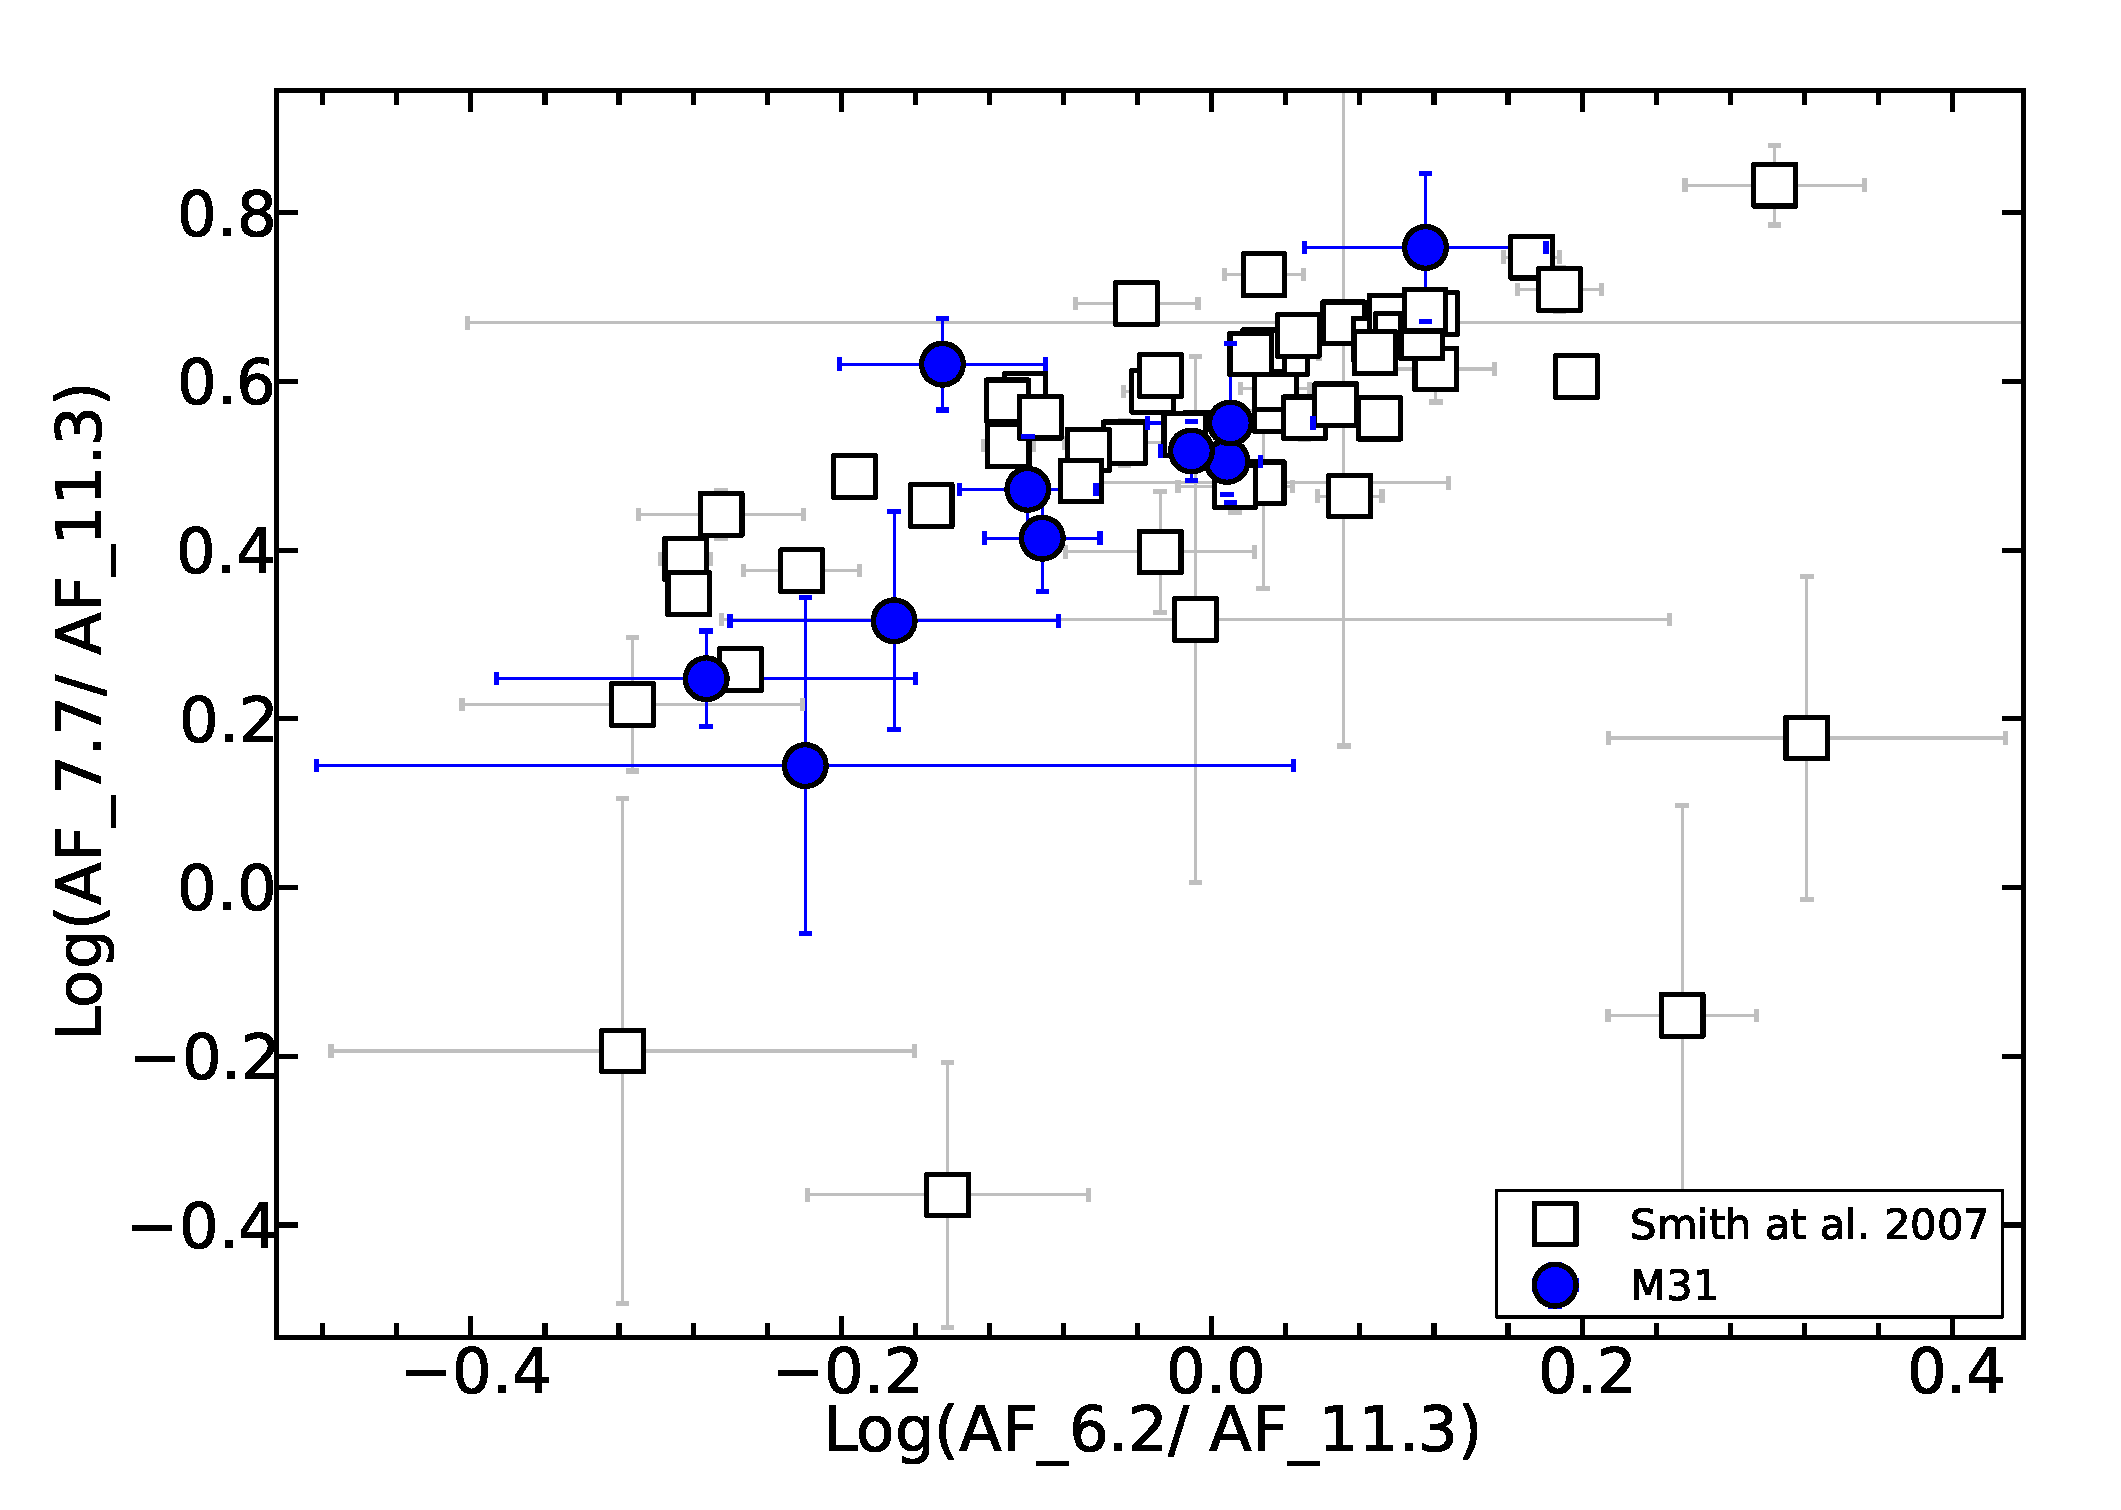
\includegraphics[scale = 0.25]{./SINGSnMy.eps}
\caption{Ratios of PAH feature fluxes (7.7~$\mu$m/11.3~$\mu$m versus 6.2~$\mu$m/11.3~$\mu$m) for 10 regions in M31.}
\label{PAHlines}
\end{figure}

\subsection{Aromatic equivalent widths versus radiation hardness}
\label{sect:eqw_rh}


\begin{figure}
\centering
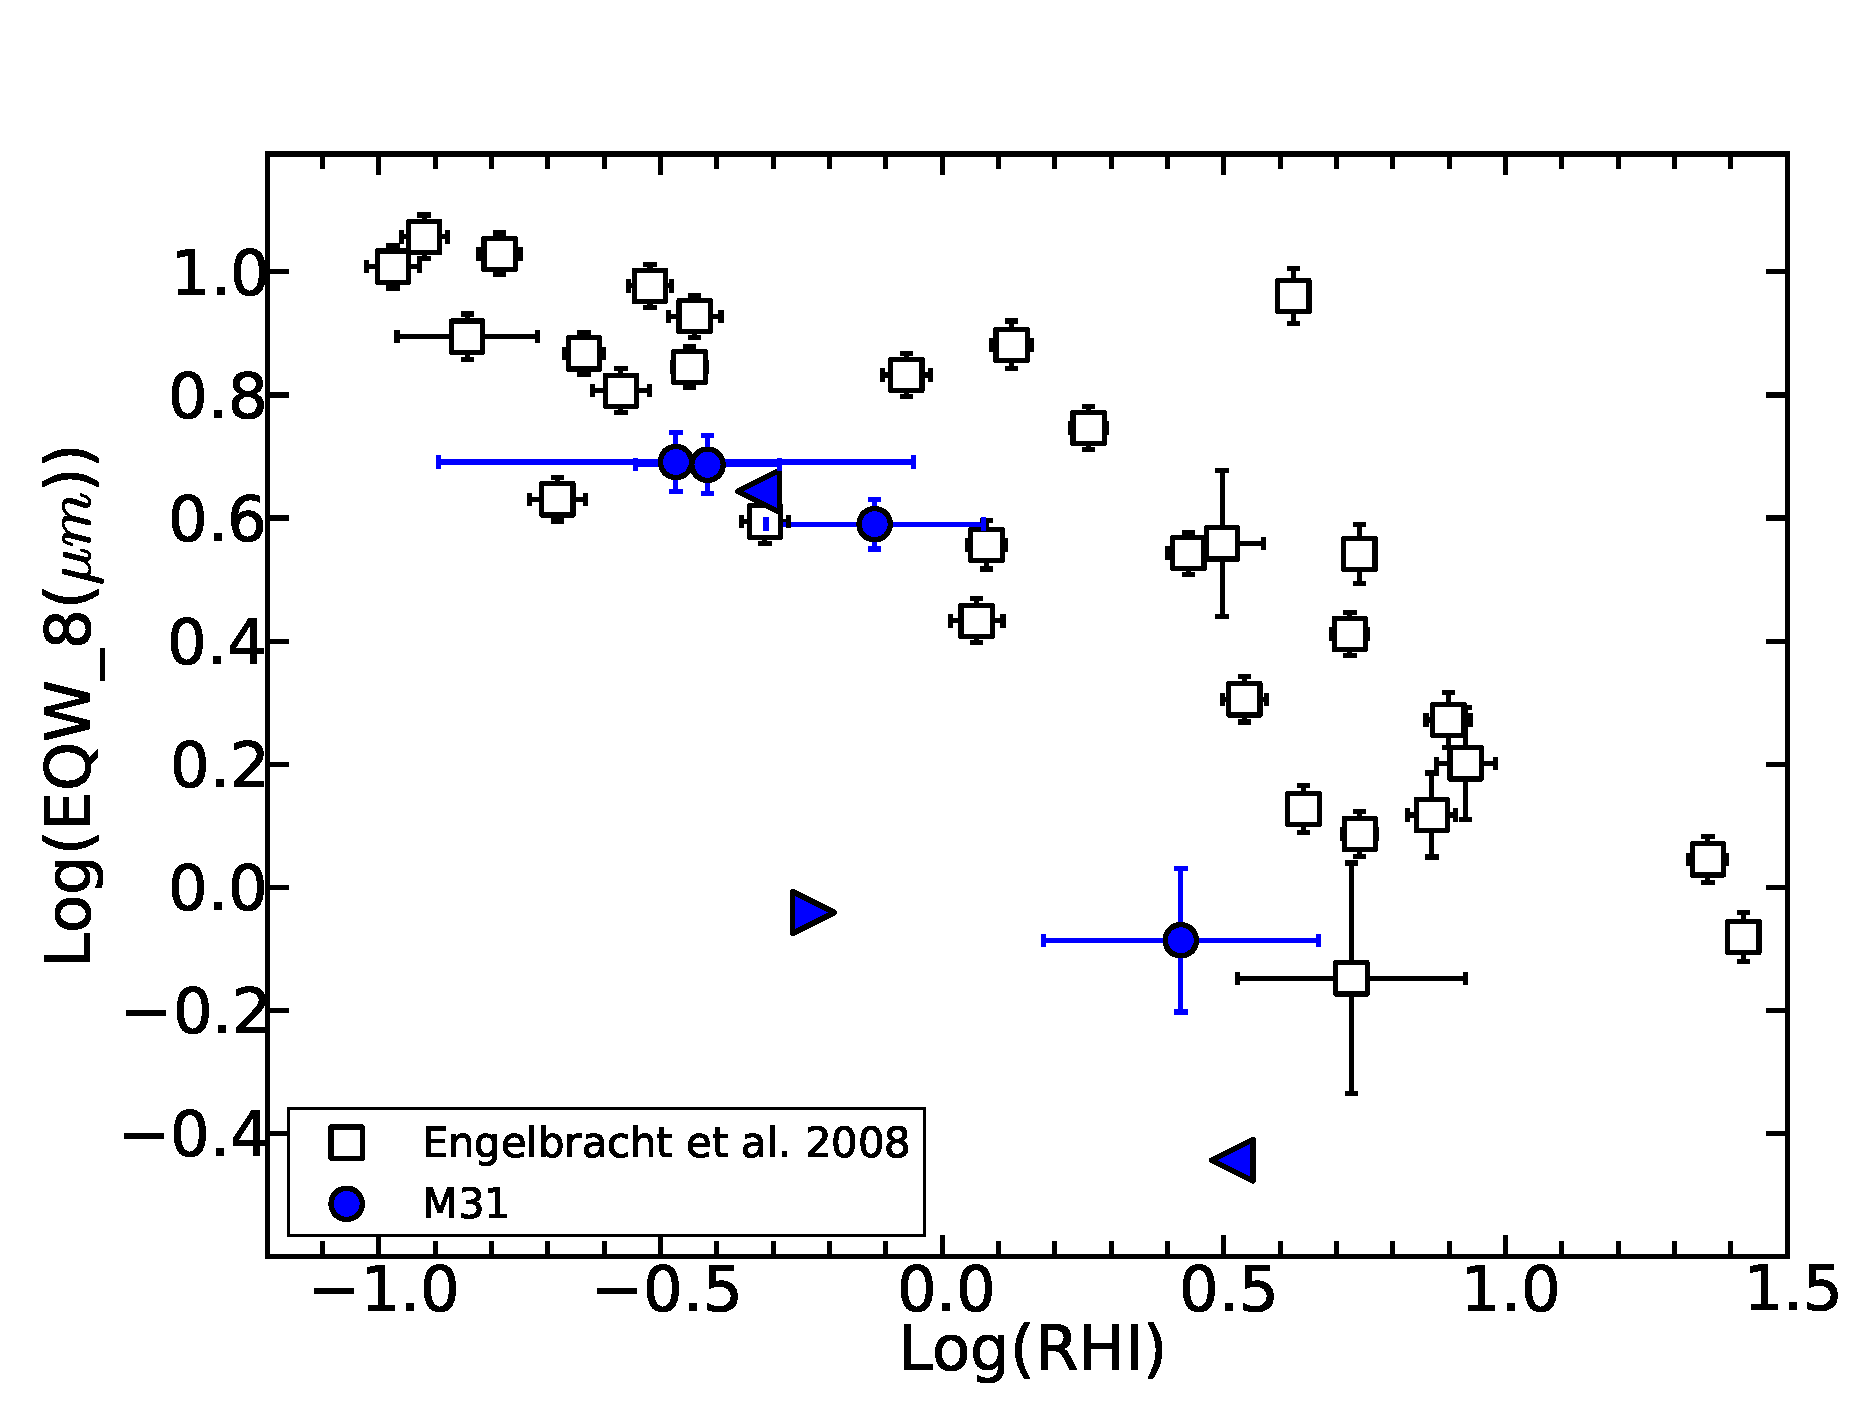
\includegraphics[scale=0.25]{./englvsmy.eps}
\caption{Equivalent width of the 8~$\mu$m aromatic feature versus radiation hardness index (RHI) for the M31 sample (blue). 
The 8$\mu$m feature is a combination of the 7.7, 8.3 and 8.6~$\mu$m PAHFIT components. 
Open squares represent the starburst galaxy sample from \citet{Engelbracht_2008}. 
For M31 spectra with undetected lines, triangles represent upper (left-pointing triangles) and lower (right-pointing triangles) limits }
\label{englII}
\end{figure}

\begin{figure}
\centering
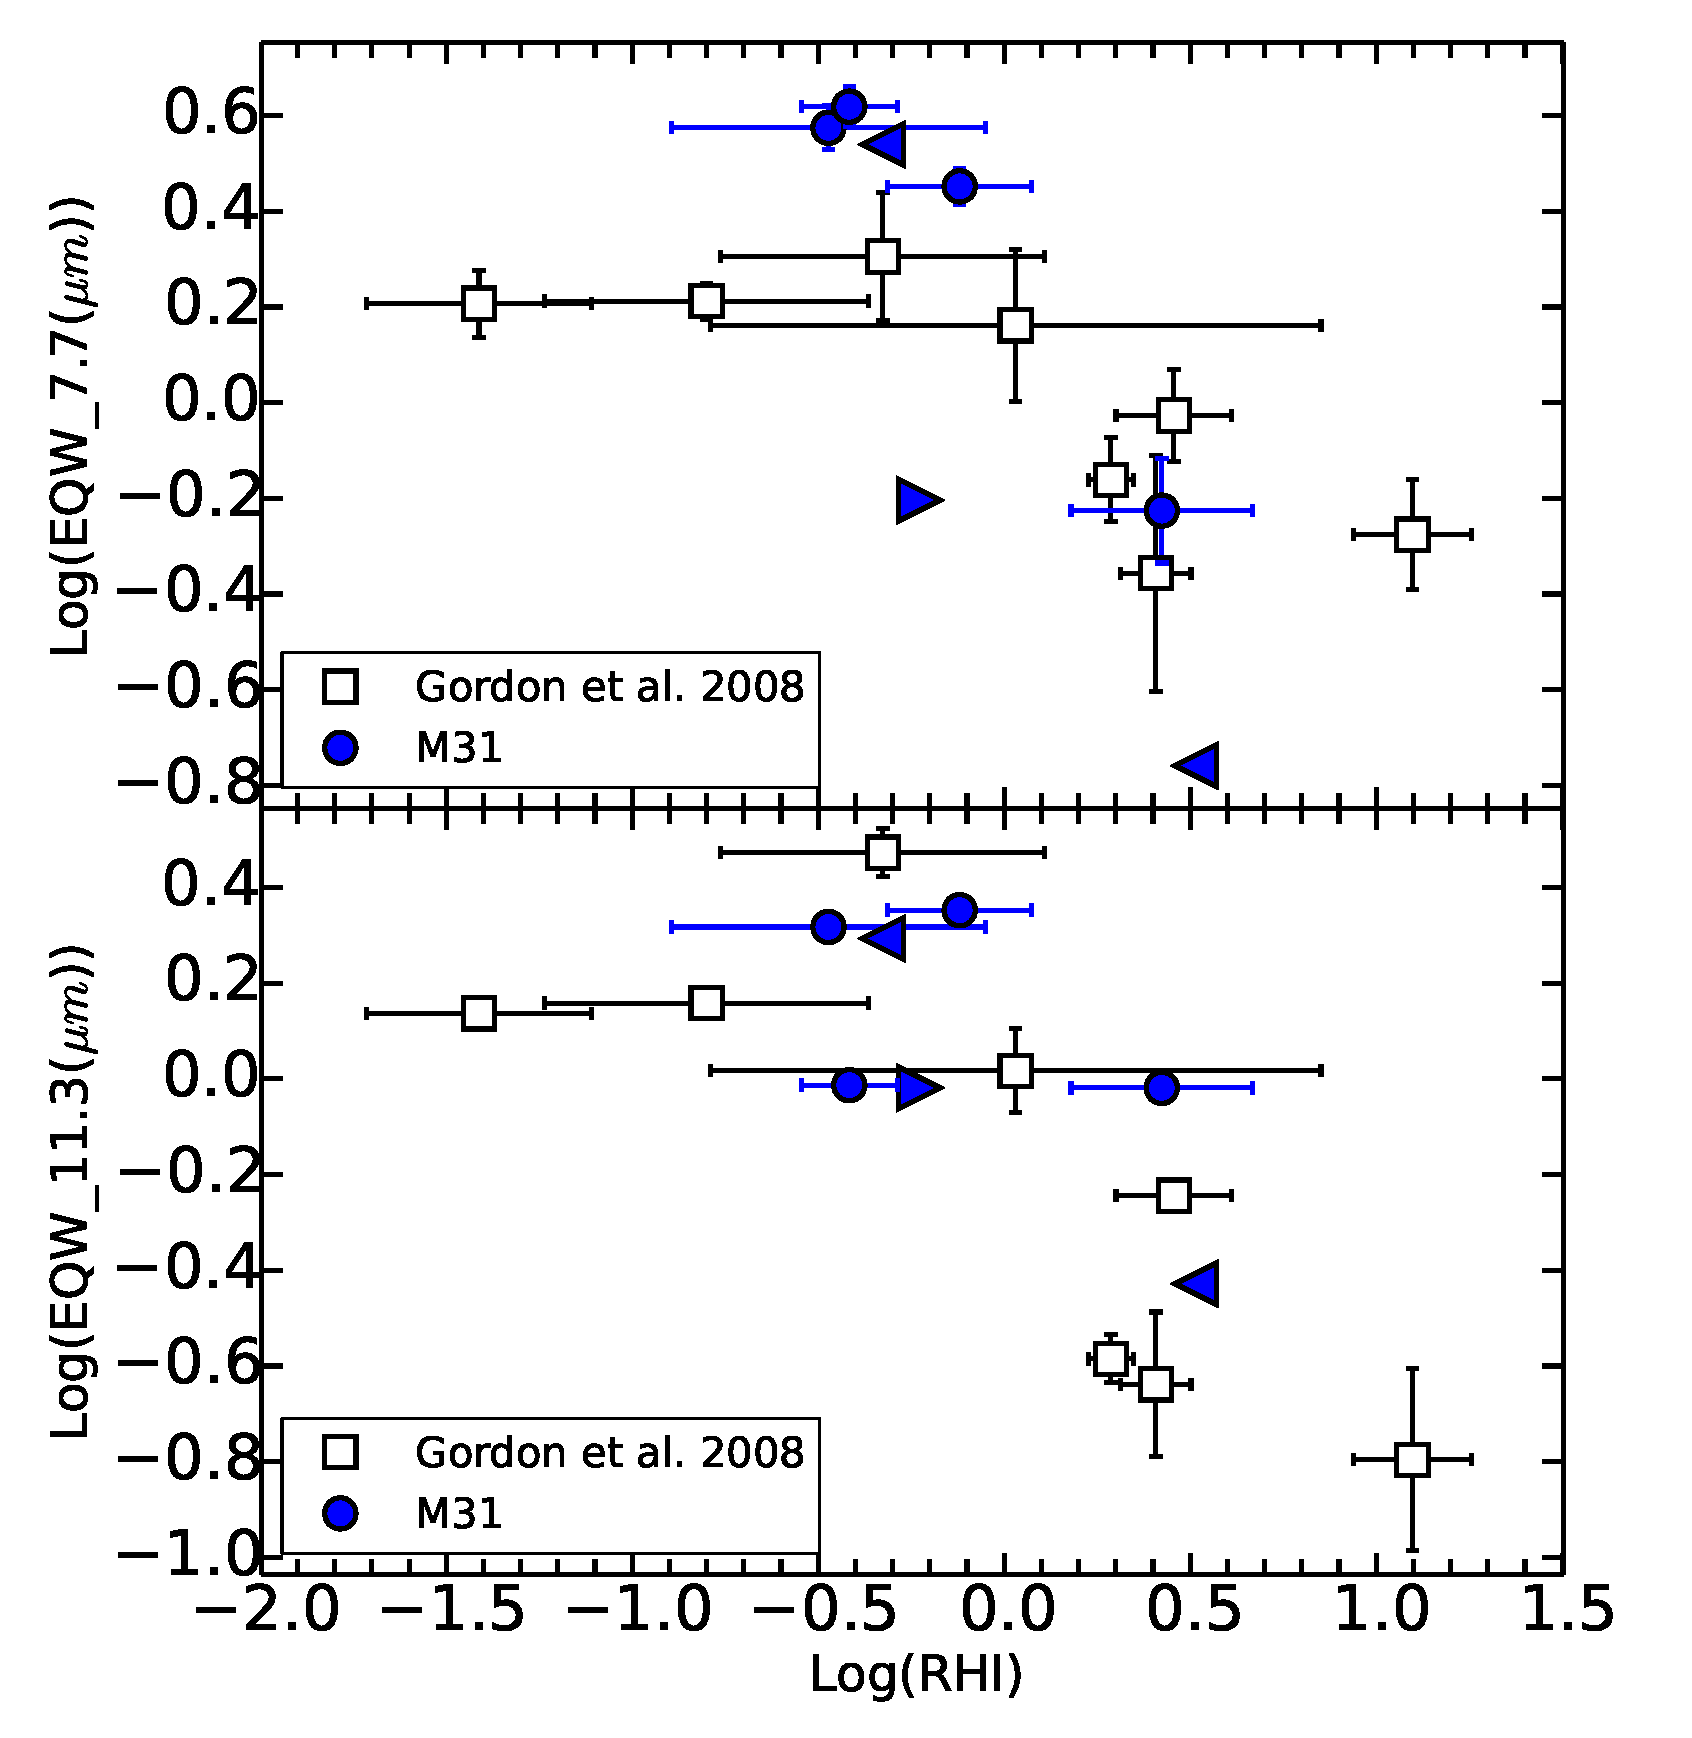
\includegraphics[scale=0.30]{./Gordvsmy.eps}
\caption{Equivalent widths of the normalized 7.7~$\mu$m aromatic feature (top panel) and 11.3~$\mu$m aromatic feature (bottom panel) versus 
radiation hardness index (RHI) for the M31 sample. Open squares represent the data from M101 by \citet{Gordon:2008lr}. 
The normalization was done by dividing each EQW by the weighted average over all regions in the respective samples. Triangles represent upper and lower limits.}
\label{gordII}
\end{figure}


As mentioned in the introduction, aromatic equivalent widths tend to show an inverse correlation with radiation hardness. 
The equivalent widths of the M31 PAH features are compared with RHI in Figures~\ref{englII} and \ref{gordII}.
For reference, we also show the starburst sample of \citet{Engelbracht_2008}, which includes 66 nearby ($2<d<250$~Mpc)
star-bursting or star-forming galaxies selected to cover a wide range in metallicity ($7.1<12+\log{\rm[O/H]}<8.9$),
and the seven H~{\sc ii} regions in M101 observed by \citet{Gordon:2008lr}, which have $8.1<12+\log{\rm[O/H]}<8.8$.
Both the  \citet{Engelbracht_2008} and \citet{Gordon:2008lr} observations were made with the SL and LL modules of IRS. 
To make a direct comparison with the M101 sample, we normalized the M31 EQWs in Figure~\ref{gordII} using the same procedure
as \citet{Gordon:2008lr}, dividing each EQW by the  weighted average over all regions in the respective samples. 
The equivalent widths seem to be decreasing with increasing radiation hardness, consistent with previous results. 
This also helps to confirm that the aromatic emission in M31 is not unusual. 


\subsection{Aromatic equivalent widths versus metallicity}
\label{sect:eqw_met}


Many studies based on ISO and {\em Spitzer} observations have reported that PAH intensity decreases with decreasing metallicity \citep{Calzetti:2010fk}. 
In addition, these studies also report a sudden drop of EQWs of PAHs around $12+\log{\rm (O/H)} \approx 8.1$. 
This has been observed amongst different galaxies \citep{Engelbracht_2008} as well as within a single galaxy \citep{Gordon:2008lr}. 
Here we investigate the relation between the PAH features and the metallicity for the M31 regions in this paper. 
As a source of metallicity measurements, we used the work of \citet{Sanders_2011} who measured spectroscopic metallicities for
more than 250 H~{\sc ii} regions using strong line diagnostics.\footnote{\citet{Sanders_2011} considered several different
calibrations for abundance diagnostics. We use the results from the method they denote ``N06 N2''  \citep{Nagao2006} because
that method has the largest sample size.} Except for regions 5 and 8, all of our mapped regions contain an  H~{\sc ii} region measured by
 \citet{Sanders_2011}, and we give the corresponding metallicity values in Table~\ref{regions}.
 For regions 5 and 8 we adopted metallicity values from the radial metallicity profile of M31 given by
 \citet{Sanders_2011}. It is well known that there are systematic differences between different 
 methods used to measure metallicities, and those in the sample of \citet{Engelbracht_2008} 
 were obtained by the direct electron temperature method  \citep{Skillman1998}.
\citet{Mitchel2014} calculated the offset between direct and strong-line measurements for M31 H~{\sc ii} region to be 
$0.35\pm0.10$. In Figure \ref{metalicityVseqw} we have corrected for this offset  by subtracting 0.35 from our metallicity values. 


\begin{figure}
\centering
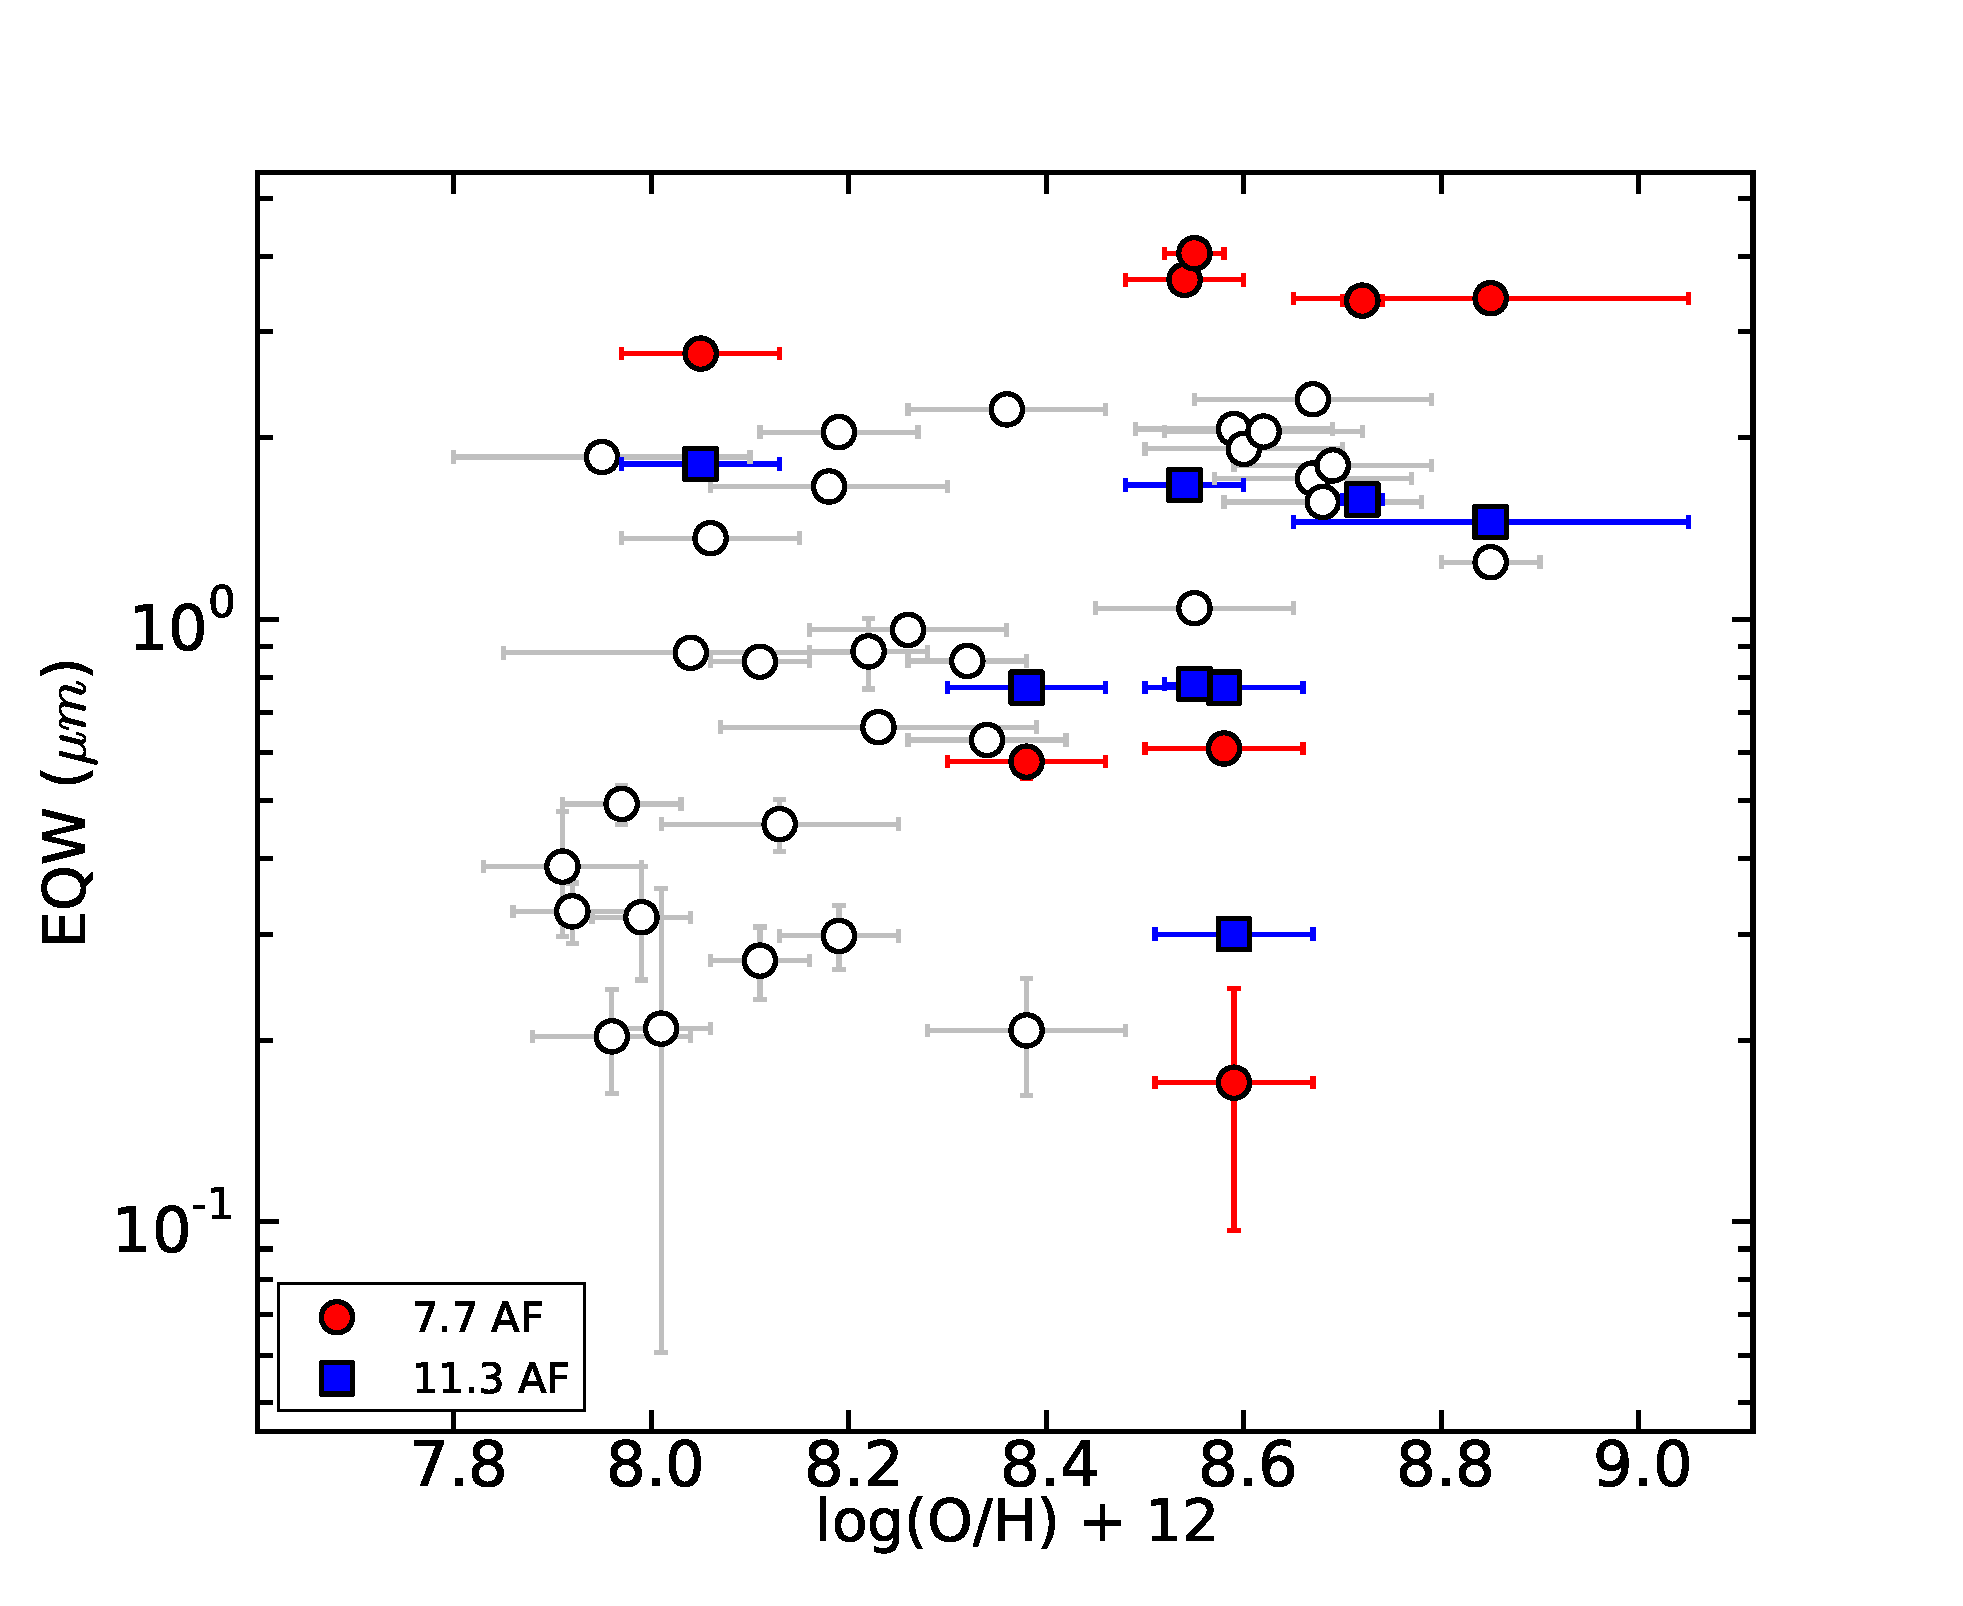
\includegraphics[scale=0.27]{./oxyvseqw.eps}
\caption{ PAH equivalent widths versus metallicity. EQWs of the 7.7~$\mu$m feature of the starburst sample from \citet{Engelbracht_2008} are plotted in open circles.}
\label{metalicityVseqw}
\end{figure}

Figure \ref{metalicityVseqw} plots the normalized EQWs of the PAH features are plotted versus the metallicity for our sample and the starburst 
galaxies of \citet{Engelbracht_2008}. The scatter in our sample is large, but the 	
equivalent widths of the 7.7 and 11.3~$\mu$m features are not inconsistent with those of \citet{Engelbracht_2008}. 
However, we do not have enough data from low-metallicity regions in M31 to observe the expected decrease of EQWs of PAH with the decreasing 
metallicity.  There do seem to be some outliers which can plausibly be due to the uncertainties  and the offset between different methods of calculating the metallicity.  
%SPW: Sec 4.2 par 4: while there's no metallicity dependence, 1 region has very low PAH.    Any idea why?  Is it just stellar light contamination, or is something fundamental happening?

%SPW: I'm not sure whether to present Fig 14 in Sec 2, but that's probably a good idea.  In Fig 14, make ticks on the vertical axis an integer number of arcsec (probably 2 or 4).
%
\begin{figure}
\centering
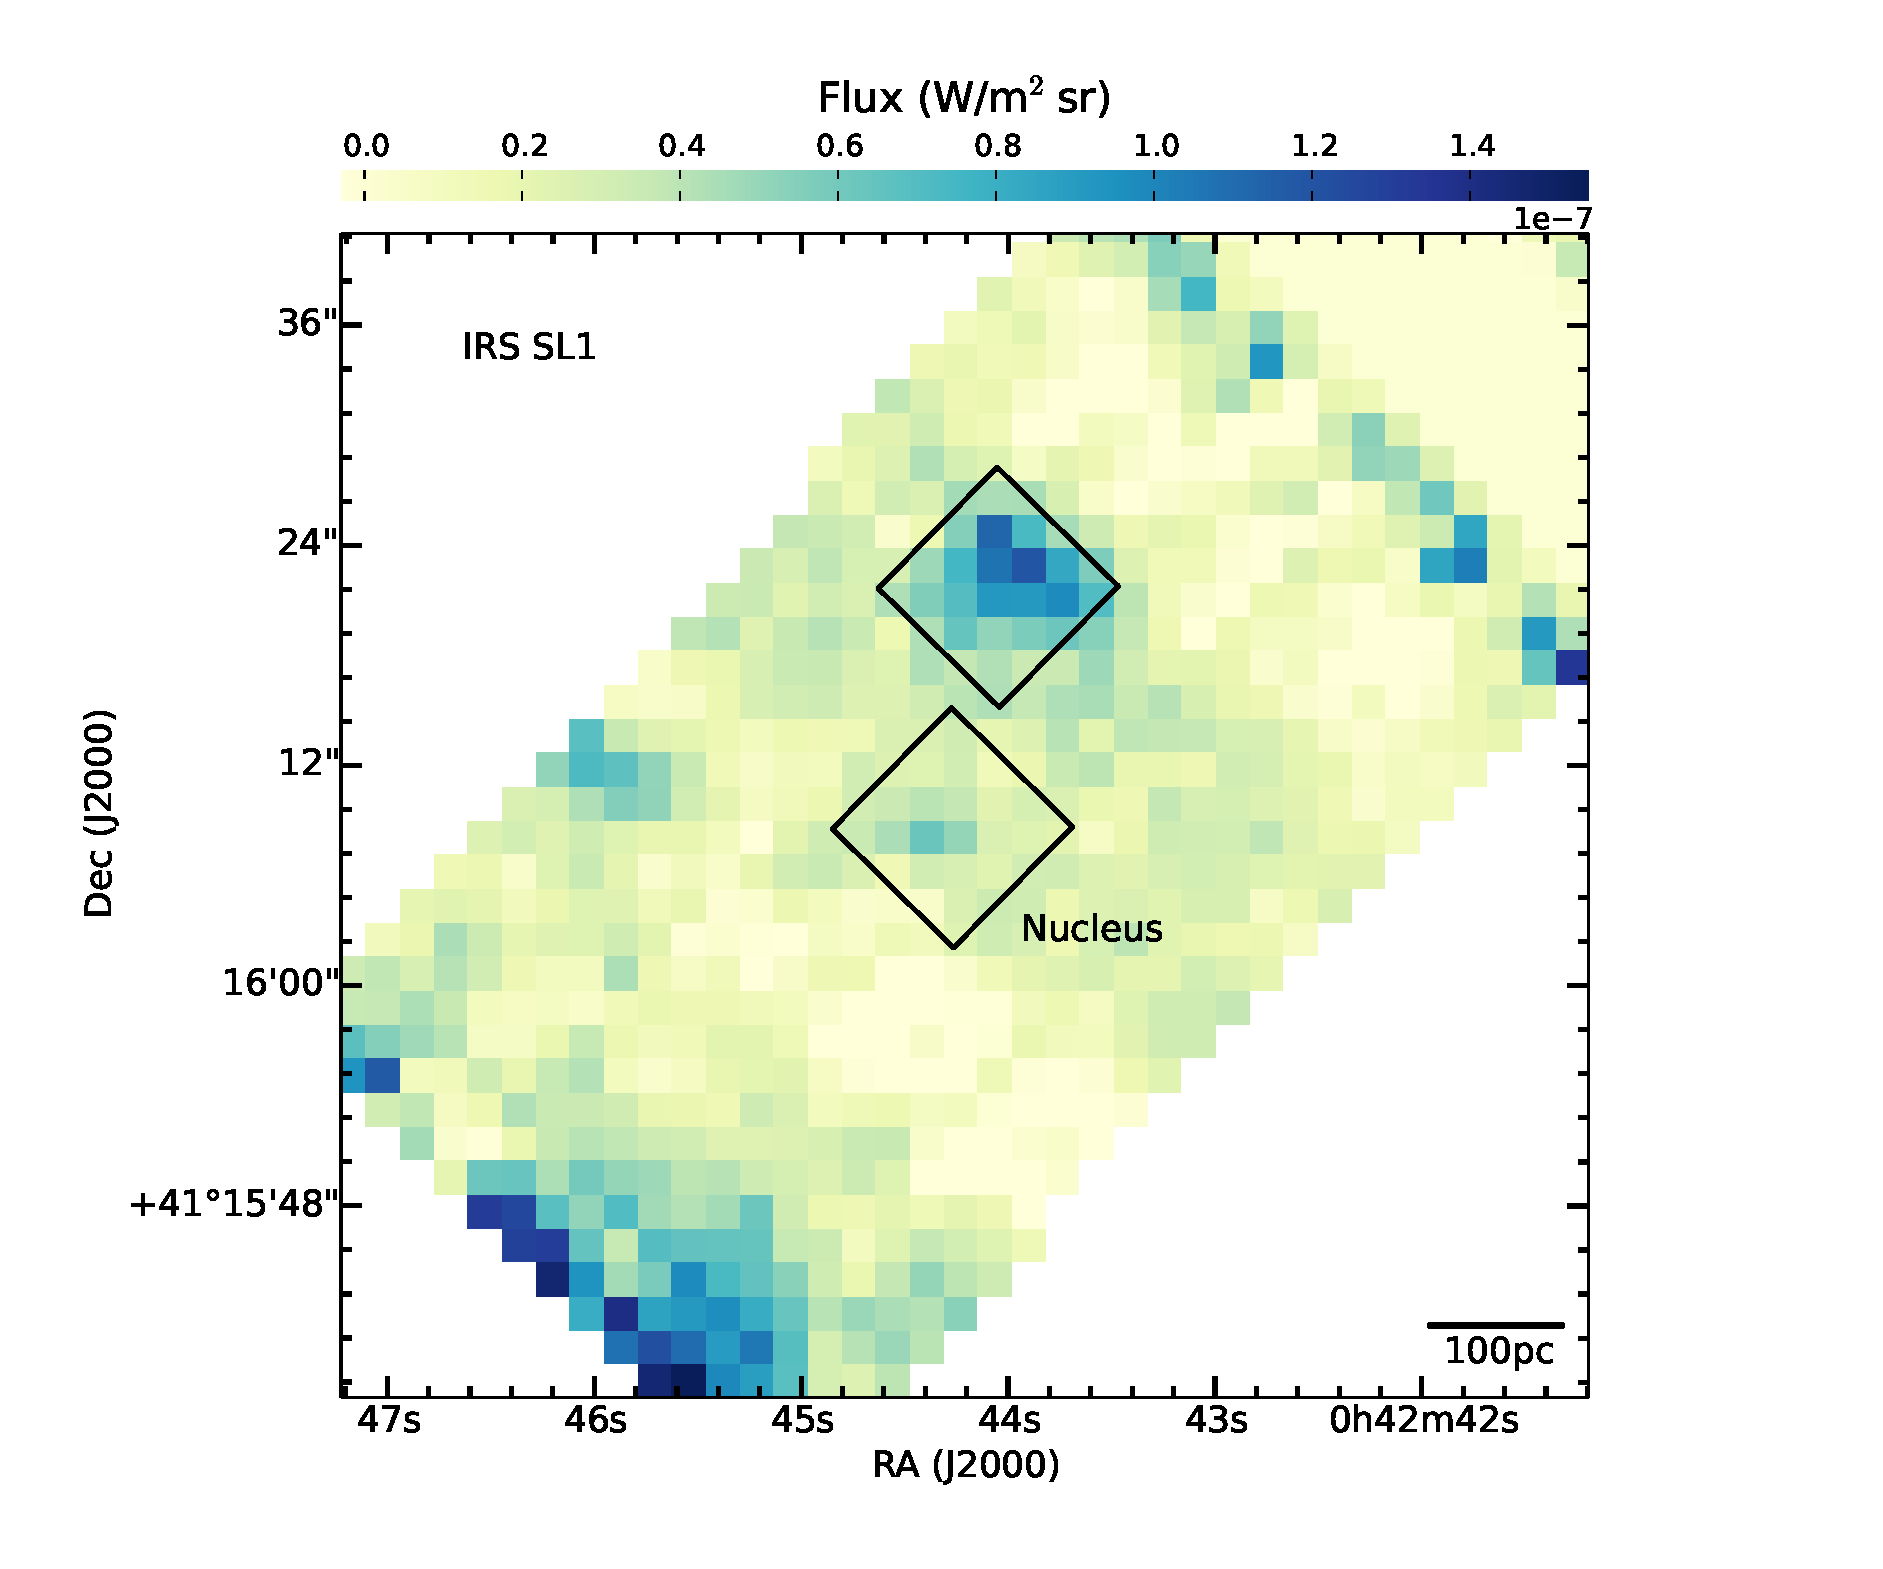
\includegraphics[width = 8 cm]{./nuc11_3.eps}
\caption{ Intensity variation of 11.3~$\mu$m emission around the nucleus of M31. 
Two black boxes are the apertures (centre and north region) used to extract spectra in Figure \ref{smithspec}. 
The centre of the nucleus is at R.A. $00^{\rm h}42^{\rm m}44\fs35$, Dec. $+41\degr16\arcmin08\farc5s$ \citep{NucleusREF}.}
\label{nuc11}
\end{figure}

\subsection{Dust properties of the nucleus}
\label{sect:nucleus}

%HAS:
%First, let me call your attention to my paper on the IRS spectrum of M81, a LINER galaxy (Smith, H.A. et al. 2010)

%It has very strong silicate emission, and curiously resembles PG quasars in this respect. 
%We presume a hot dusty torus. We also image the dust around the nucleus; we see 11.3, 12.7 and 16.5 PAH, but only barely the 6.3 and 8.6 features. 
%
%I guess the nuclear spectrum is in your Figure 15 - why did you not try to fit it with PAHFIT too?  It looks to me like it has a weak 20um silicate bump too.
% Why not include the nuclear region in Tables 2,3&4?  I did not understand the reason for leaving it off.  Also please add the limit for the [Ne V] detection - it might still be a useful ratio with [Ne II] and the PAH lines.  It looked to me like there was some hint of the H2 12.28um line in some regions.... maybe add that limit too, though I was surprised

\begin{figure*}
\centering
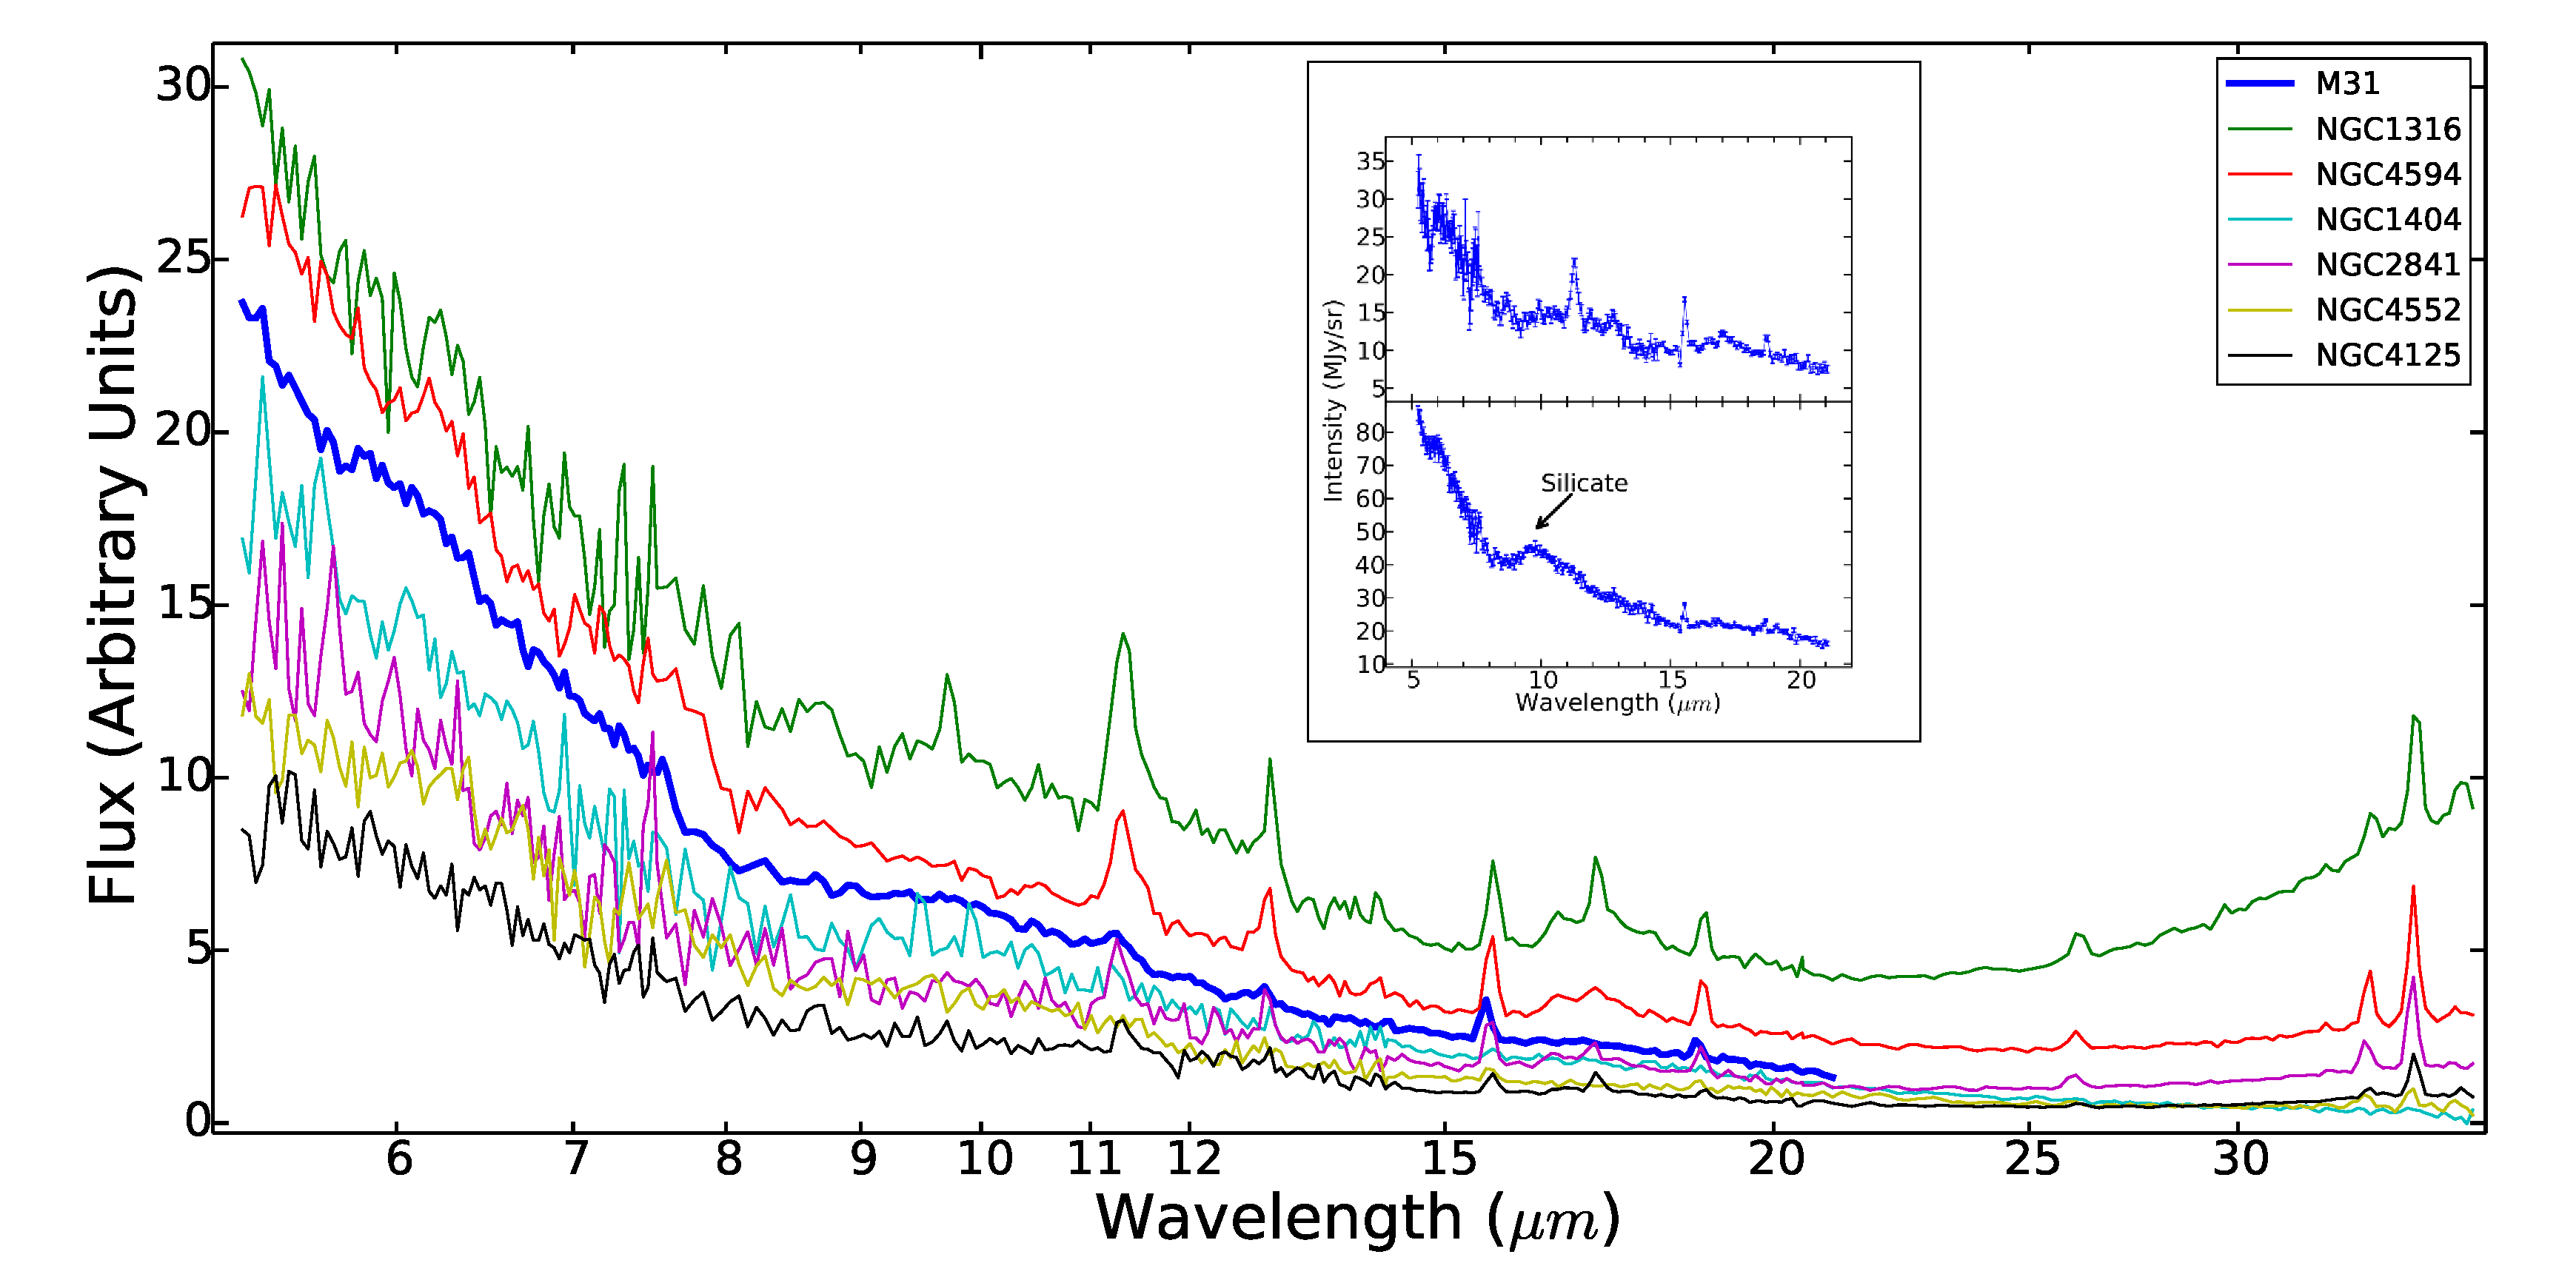
\includegraphics[height = 8 cm]{./SINGSspec.eps}
\caption{Mid-infrared spectrum of the nucleus of M31 (blue) over-plotted with spectra extracted close to the nuclei of 6 nearby galaxies which have 
AGN activity \citep{Smith:2007lr}. NGC 4552, NGC 1404 and NGC 4125 are elliptical galaxies and NGC 4594 and NGC 2841 are spiral galaxies. 
NGC 1316 is a lenticular galaxy. The inset shows the spectra extracted from the centre region of the M31 nucleus (bottom) and from the north region (top) 
shown in Figure \ref{nuc11}.}
\label{smithspec}
\end{figure*}

The mid-infrared spectra of the nucleus from both {\em Spitzer} and ISOCAM (Figure~\ref{ISOnIRS}) show similar characteristics: a blue
continuum, PAH features weak or absent at 6--8~$\mu$m  but detectable at 11.3~$\mu$m, and detectable atomic fine structure lines.
Comparing the M31 nuclear spectrum with the nuclear spectra from the SINGS sample given by \citet{Smith:2007lr}, we found
six other galaxies with similar spectral shapes. These include three elliptical galaxies, two spirals, and a lenticular;
the IRS spectra for these galaxies were extracted over areas ranging from 2 to 8 kpc$^2$.
The SINGS papers \citep{kennicutt03,Smith:2007lr, moustakas2010} are in some disagreement over the
exact nuclear spectral types of these six galaxies. All are classified as some form of low-luminosity AGN
\citep[luminous AGN were intentionally omitted from the SINGS sample][]{kennicutt03}, but they are
by no means the only LLAGN in the SINGS sample.
Figure~\ref{smithspec} shows the M31 nuclear spectrum with the comparison spectra.

% this needs work
A suppression of 6--8~$\mu$m features has also been observed in other nearby star-forming galaxies with a low-luminosity AGN \citep{Smith:2007lr},
and those authors  argue that this variation could be used to detect weak AGNs in dusty galaxies where optical diagnostics are not available. 
One explanation for this behaviour is that the AGN environment can selectively destroy the ionized or small PAH molecules which contribute to the 6--8~$\mu$m 
features (whereas larger, neutral PAHs contribute to the 11.3~$\mu$m feature). Another argument is that the AGN is unrelated or partially responsible for the PAH spectra alterations. \citet{Smith:2007lr} 


%MLNA: Sec 4.3 -- I see the North region, but where is the South East one -- can it be indicated in Fig 14 somehow,  to distinguish from the noise at the edge of the mosaic?
%SPW: First of all, I think the additional spectra of "nucleus" and "north" needed to be introduced back in Sec 2.  Presumably "bulge" is the usual 20"x30" region.  You give north and nucleus in pixels, but what are they in arcsec?  Pixels differ between SL and LL.  I'd like to see the two small regions included as table rows and in Fig 8/9 with PAHFIT, just like all the other spectra.  The main part of Fig 15 can remain as is, though probably the ordinate should be logarithmic.

%SPW: Sec 4.3 par 3: are the nucleus and north sources spatially resolved, or are they consistent with point sources?
%
Figure \ref{nuc11} shows the integrated intensity map of 11.3~$\mu$m emission around the nucleus. It can be observed that the majority of the 11.3~$\mu$m 
emission is coming from two regions (North and South East) around the centre of the nucleus and not from the centre. To study this further, we extracted two 
spectra, one from the centre and one from the North region using a $5 \times 5$ pixel square aperture as shown in Figure \ref{nuc11}. The spectrum extracted 
from the North region shows a strong 11.3~$\mu$m peak as expected and no significant emission from 6--8~$\mu$m features (Figure \ref{smithspec}, inset). 
On the other hand the centre shows no PAH emission (Figure \ref{smithspec}) but silicate emission around 9.7~$\mu$m which is not present in the North spectrum. 
To investigate whether there are any other regions that show silicate emission close to the nucleus, a continuum subtracted image was produced which shows the 
9--11~$\mu$m integrated emission intensity (see Figure \ref{silicate}). This emission map shows that only the exact centre of the nucleus contributes 
to the silicate emission. 

\citet{Spoon2007} report that galaxies which have AGN activity show silicate emission around 9.7~$\mu$m.
In the unified model of AGNs, an edge on view through cool dust (type 2 AGNs) in the torus causes silicate absorption whereas a face-on view (type 1 AGNs) 
shows silicate emission \citep{AGNtypes1995}. The latter could be the reason for silicate emission of M31 if it holds a Seyfert-like AGN. 
But the mid-IR spectra do not contain forbidden atomic lines such as [Ne~{\sc v}] and [S~{\sc iv}] which are indicative of such an active nucleus \citep{AGNref}.

 Alternatively, the silicate emission is not directly associated with the torus but rather originate in the optically thin hot dust around the torus \citep{Mason2012}. 
 The first detection of such silicate emission is reported in \citet{Sturm2005} from the low-ionization nuclear emission-line region (LINER) galaxy NGC 3998. 
 LINERs are powered by accretion onto massive black holes and due to the low accretion rates these are classified as the low-luminosity AGNs \citep{Kewley2006}. 
 \citealt{Mason2012} has observed that this 9.7~$\mu$m silicate emission is present in many LLAGNs. They also have explained that these objects cannot 
 host a Seyfert-like obscuring torus because of their optically thin dust and low dust-to-gas ratio. By taking all these into account, we can suggest that M31 
 hosts a low-luminosity AGN. 

%HAS: I was trying to think more about the significance of the result. Although indeed some quasars and LINERS have silicate emission, I don't think your conclusion in the abstract that the emission "provides evidence for a LLAGN" is correct as worded -  3C273 has silicate emission too.  It might be useful to tabulate the masses of the black holes in each of the 6 comparison galaxies, to see whether spectral similarities (or differences) can be attributed to the quiescent AGN, as you suggest, of whether circumnuclear star formation or other things might play some role.
 
 %SPW: Sec 4.3 par 5: luminosity needs a sentence or maybe two at most, not a par.
Also, the bolometric luminosity of the nucleus was calculated to be (value goes here erg/ s) using the 12~$\mu$m flux using the method described in \citet{luminosity}. This value is closer to that of other LLAGNs.


\begin{figure}
\centering
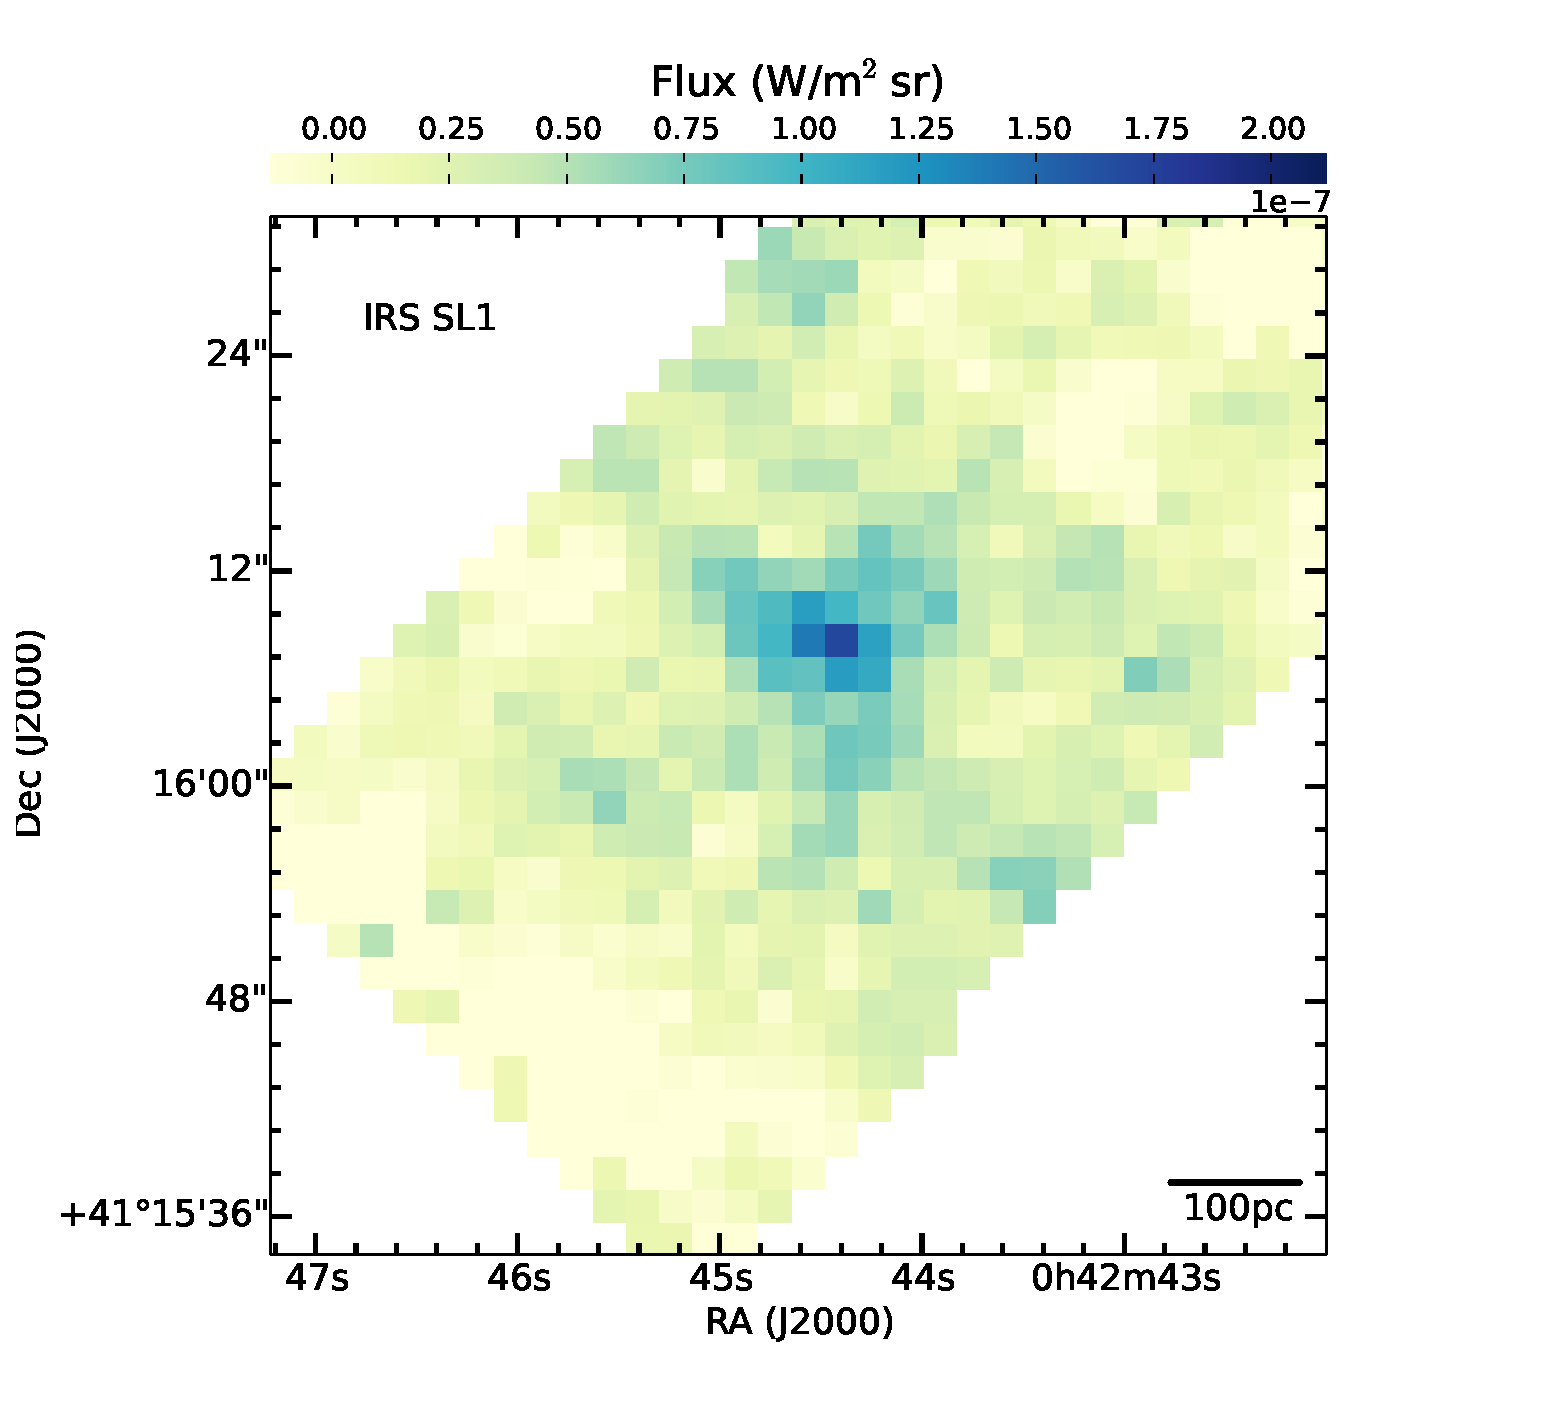
\includegraphics[scale = 0.3]{./NUCsilicate.eps}
\caption{The integrated strength of the silicate emission (from 9 to 11~$\mu$m) near the M31 nucleus.}
\label{silicate}
\end{figure}
